\section{Umsetzung der Aufgaben des Meta-Bereichs}
Dieser Abschnitt beschäftigt sich mit unserer Umsetzung der Aufgaben des Meta-Bereichs. Unser Ziel war es, nach jedem Durchlauf zu "lernen", indem man das vorherige Handeln speichert, evaluiert und dies beim wiederholten Durchlauf berücksichtigt.

\subsection{Meta}
Die Hauptklasse \texttt{Bambird}, die sich im Ordner \texttt{main} befindet, stellt die Verbindung vom Client zum Server her und ihre Instanz entspricht unserer Version des intelligenten Agenten \glqq BamBird \grqq, der Angry Birds spielt. \\
Darin wird ein Objekt der Klasse \texttt{Meta} angelegt, wo das eigentliche Zusammenspiel aller im vorigen Kapitel genannten Komponenten (jedoch ohne Physik-Simulation) stattfindet -- sie entspricht also der tatsächlichen \glqq Main-Klasse\grqq. Zur Veranschaulichung des Aufbaus der Hauptmethode \texttt{startMeta}, wird dessen Ablauf in folgendem Pseudocode \ref{meta} dargestellt:

\begin{algorithm}[H]
  \begin{algorithmic}[1]
  \Loop
  	\If{GameState != Playing}
  		\State choose new Level
  	\EndIf
  	\State take a screenshot from the scene and analyse
  	\State generate plans
  	\State choose one plan to be executed as a shot
  	\State execute chosen shot
  	\State add shot to the shot-list of the current level
  	\If{GameState == WON or GameState == LOST} \\
  		\hspace{2.5em} add level to database
  	\EndIf
  \EndLoop
  \end{algorithmic}
  \caption{Meta \label{meta}}
\end{algorithm}

Die Schleife läuft ständig bis das Spiel zu Ende ist bzw. die vom Wettbewerb vorgegebene Zeit abgelaufen ist. Das Level wird einmal durchgespielt und anschließend mit den ausgeführten Schüssen in einer Datenbank abgespeichert. Erst wenn der Spielstatus nicht mehr auf \glqq Playing\grqq steht, wird ein neues Level ausgewählt und das gleiche Prozedere folgt. \\
Im Folgenden wird genauer auf unsere Umsetzung der einzelnen Komponenten des Meta-Bereichs eingegangen.

\subsection{Level und Datenbank}

\subsubsection{Level} \label{Level}
Zur Speicherung der ausgeführten Aktionen wird eine Datenbank benötigt. Doch bevor man solch eine für die verschiedenen Level bauen kann, müssen die grundlegenden Informationen kompatibel sein: das Level selber. Somit besteht die Fragestellung also darin, welche Informationen über ein Level benötigt werden. \\ Unsere Java-Klasse \texttt{Level} befindet sich im Ordner \texttt{Meta}. Diese besteht aus
\begin{itemize}
\item der Level-ID, 
\item den geschätzten maximal zu erreichenden Punkten dieses Levels, 
\item den tatsächlich erreichten Punkten, 
\item der Anzahl der gespielten Durchgänge und 
\item einer Liste von ausgeführten Schüssen.
\end{itemize} 
Das Abspeichern der Schüsse erfolgt in Form der Klasse \texttt{Triplet}, die sich auch im \texttt{Meta}-Ordner befindet. Hierbei wird neben dem eigentlichen Schuss (\texttt{shot}) zusätzlich noch das anvisierte Zielobjekt (\texttt{target}) und die allein aus diesem Schuss erreichten Punkte (\texttt{damagePoints}) gespeichert, welche später in der \texttt{ShotSelection} (siehe Kapitel \ref{ShotSelection}) relevant sind. \\
Die \texttt{Level}-Klasse an sich dient als Grundlage und Speicherobjekt und enthält dementsprechend nur wenige Methoden. 

\subsubsection{Datenbank}
Nach jedem Durchlauf eines Levels werden die oben genannten Informationen in ein \texttt{Level}-Objekt gespeichert, wobei jedes einzelne davon wiederum in eine Datenbank hinzugefügt wird. Die dazugehörige Klasse ist unter \menu{ database > LevelStorage} zu finden. \\
Der Ordner \texttt{database} enthält ebenso eine enum-Klasse \texttt{LevelState}, welche wir nur zur Markierung der Level einsetzen, weiterhin jedoch keine höhere Verwendung findet. \\ 
Die \texttt{LevelStorage} besteht aus einer privaten Map, die die \texttt{Level} und den dazugehörigen \texttt{LevelState} beinhaltet. Zusätzlich enthält die Klasse eine öffentliche Liste aus Integer, die in der gleichen Reihenfolge wie der Map die Level-IDs der gespielten Level speichert, sodass man von au\ss en schnell auf die Information zugreifen kann, welche Level bereits gespielt wurden, sowie den Index der Level leichter abfragen kann. \\
Beim Speichern der Level muss darauf geachtet werden, dass man die Level nicht doppelt speichert im Falle eines wiederholten Versuchs. Daher prüfen wir in unserer öffentlichen Methode \texttt{addLeveltoStorage}, ob das übergebene Level bereits in der Datenbank enthalten ist. Falls es einen Eintrag mit dieser Level-ID gibt, wird die Hilfsmethode \texttt{updateLevelInfo} aufgerufen, welche nur die geänderten Einträge aktualisiert, anstatt einen komplett neuen Eintrag zu erstellen. \\
Die \texttt{LevelStorage} ist in der Evaluation von gro\ss er Bedeutung und wird in den Klassen der nachfolgenden Kapitel verwendet.

\subsection{Level Selection}
Die Klasse \texttt{LevelSelection}, die sich im Ordner \texttt{Meta} befindet, ist für die Levelauswahl zuständig und wird zu Beginn der Schleife aus dem \texttt{Meta}-Code aufgerufen (siehe Pseudocode \ref{meta}). Sie hält die Information über die gesamte Anzahl der zu spielenden Level und über das aktuelle Level selbst, das gerade gespielt wird. \\ 
Die Hauptmethode \texttt{selectNextLevel} lässt alle Level beginnend mit einer zufällig ausgewählten Levelnummer der Reihenfolge nach durchspielen. Sobald all diese einmal vollendet wurden, muss nun entschieden werden, welche Level in welcher Reihenfolge und wie oft wiederholt werden sollen. \\
Die Auswahl erfolgt nach einer simplen Wahrscheinlichkeitsberechnung, welche aussagt, wie wahrscheinlich es ist, mit einem bestimmten Level noch mehr Punkte erzielen zu können bzw. sich in diesem Level zu verbessern:  \\
$$ Probability = 1 - ( actualScore / maximalReachableScore ) $$
Wir richten uns also danach, wie viele Punkte wir von der maximal erreichbaren Punktzahl im ersten Durchgang bereits abdecken konnten. Das Level mit der höchsten Wahrscheinlichkeit wird dann ausgewählt. \\
Eine Besonderheit gibt es für verlorene Level, welche als erste ausgewählt werden, denn ihre erbrachte Punktzahl hat den Wert 0 und somit beträgt die Wahrscheinlichkeit, sich zu verbessern, 1. Da man für jedes Level im Durchschnitt mindestens drei Minuten erhält \footnote{\url{https://aibirds.org/angry-birds-ai-competition/competition-rules.html} (zuletzt abgerufen: 05.09.2017)} und wir von einer Durchschnittsspieldauer von 1 - 1,5 Minuten pro Level ausgingen, entschieden wir uns, die verlorenen Level zunächst höchstens zweimal wiederholen zu lassen. Falls die Quote der verlorenen Level im Bezug auf die Gesamtanzahl der zu spielenden Level dann immer noch zu hoch ist, soll der Agent ein weiteres verlorenes Level auswählen. In unserem Fall haben wir die Grenze auf 15\% gesetzt, d.h. der Agent würde bei einer Gesamtanzahl von 21 Level einen erneuten Versuch an verlorenen Level starten, wenn mehr als 3 Level noch verloren sind. Falls dann immer noch nicht alle Level gewonnen wurden, sollen diese ignoriert werden. \\ 
Zur Veranschaulichung, wie der Algorithmus implementiert werden soll, dient der Pseudocode \ref{lvlSelec}. Hierbei haben wir einen boolean-Wert \texttt{ignoreLostLevels} integriert, der erst dann auf \textbf{true} gesetzt wird, wenn alle verlorenen Level zweimal wiederholt wurden und die Quote der verlorenen Level unter 15\% beträgt. Dieser Wert wird dann in der zweiten if-Schleife geprüft. \\
\begin{algorithm}[H]
  \begin{algorithmic}[1]
  	\State \textbf{boolean} \textit{ignoreLostLevels} = false
  	\\
  	\State \funccall{calculateProbabilities}() \Comment{calculates the probability for every level}
  	\\
  	\If{lost levels exist}
  		\If{all lost levels were repeated twice}
  		 	\If{Amount of lost levels > 15\% of total number of levels} 
  		 		\hspace{\algorithmicindent}  \Return \funccall{next lost level} \Comment{redo the lost levels one more time}
			\Else  
				\State \textit{ignoreLostLevels} = true
  		 	\EndIf
  		\Else
  			\Return \funccall{next lost level that has not been played twice yet}
  		\EndIf
  	\EndIf
  	\\
  	\If{no lost levels exist \textbf{or} \textit{ignoreLostLevels} == true}
		\Return level with the highest probability  	
  	\EndIf
  \end{algorithmic}
  \caption{Level selection after every level was played at least once \label{lvlSelec}}
\end{algorithm}

\subsection{Shot Selection} \label{ShotSelection}
Um bei wiederholten Versuchen von Level nicht ständig dieselben Schüsse zu nehmen und unsere Spieltaktik zu verbessern, kommt nun die Schussauswahl ins Spiel. Dafür bekommt unsere Klasse \texttt{ShotSelection}, die sich ebenfalls im \texttt{Meta}-Ordner befindet, von der Strategie-Gruppe für jeden Vogel eine Liste von Zielobjekten (\texttt{Targets}), auf die der Vogel schie\ss en soll (siehe Methode \texttt{chooseShotWithOneList}). Eines davon wandeln wir dann in ein \texttt{Shot}-Objekt um und der Agent kann den Schuss dann im Spiel ausführen. Nachdem ein Schuss getätigt wurde, wird dieser dann für das entsprechende Level in eine Liste von Schüssen gespeichert (vgl. Kapitel \ref{Level}). \\
Zu den jeweiligen \texttt{Targets} wird eine Konfidenz zwischen 0 und 1 von der Strategie-Gruppe mitübergeben, nach welcher der auszuführenden Schuss ausgewählt wird. 

\subsubsection{Verhindern von Wiederholen von Schüssen}
Es besteht die Gefahr, dass immer derselbe Schuss genommen wird. Dies kann eintreten, wenn ein Schuss einer hohen Konfidenz zugeordnet wird, im echten Spiel jedoch wenig oder sogar keine Wirkung auf die Schweine und Strukturen hat. Da nach jedem Schuss neue Pläne in Bezug auf den jetzigen Stand der Umgebung generiert werden und sich die Szene in dem Fall nicht verändert, erhalten wir von der Strategie-Gruppe stets die gleiche Liste von Plänen. Würden wir also den Algorithmus ohne Einschränkung lassen, würde immer das Zielobjekt mit der höchsten Konfidenz ausgewählt werden, welches bei gleichen Szenen immer denselben Schuss entspricht. 
Somit haben wir einen Algorithmus integriert, der in Bezug auf die noch übrig gebliebenen Vögel entscheidet, ob der Schuss ein zweites Mal probiert werden soll, da es auch oft der Fall ist, dass der erste Schuss die Gebäude zum Wackeln gebracht hat und ein zweiter Schuss auf das gleiche Ziel den Endstoß bringt. Dies lassen wir jedoch nur zu, wenn die Chance noch hoch genug ist, mit den restlichen Vögeln das Level trotz eines zweiten Fehlschusses noch gewinnen zu können. Dies wird in folgendem Pseudocode \ref{ShotSelec} veranschaulicht, wo wir uns nach der Gesamtzahl der Vögel richten: \\
\begin{algorithm}[H]
  \begin{algorithmic}[1]
  \If{shotCandidate.equals(previousShot)}
  	\If{(totalBirdAmount <= 3 \&\& executedShots >= 2) \textbf{or} \\ 
  	\hspace{\algorithmicindent} (totalBirdAmount > 3 \&\& previousPreviousShot.equals(previousShot))}
  	\\ \hspace{2.5em} \funccall{choose another shotCandidate}
  	\Else \\
  		\hspace{2.5em} \funccall{proceed with the current shotCandidate}
  	\EndIf
  \EndIf
  \end{algorithmic}
  \caption{Prevention of endless repetition in ShotSelection \label{ShotSelec}}
\end{algorithm}

\begin{table}[H]
\begin{itemize}
\item \textit{shotCandidate}: der zu prüfende Schuss, der ausgeführt werden soll 
\item \textit{previousShot}: der Schuss, der als letztes tatsächlich ausgeführt wurde
\item \textit{previousPreviousShot}: der Schuss, der vor dem zuletzt ausgeführten Schuss ausgeführt wurde
\end{itemize}
\end{table}

In unserem Algorithmus wird also nur derselbe Schuss im Fall von mehr als 3 Vögel noch einmal ausgeführt, wenn die zwei Schüsse vor dem aktuellen Schuss nicht schon identisch waren, d.h. ein Schuss darf nicht mehr als einmal wiederholt werden. Im Falle von höchstens drei Vögel, wird ein anderer Schuss ausgewählt, wenn es sich gerade um den letzten Vogel handelt.

\subsubsection{Schussevaluation}
Falls das Level bereits gespielt wurde, überprüfen wir zunächst, ob der ausgewählte Schuss beim letzten Durchgang ebenfalls schon an dieser Stelle zum Einsatz kam und ob er \glqq gut\grqq oder \glqq schlecht\grqq war. Dementsprechend soll ein anderes Zielobjekt ausgewählt werden, wenn der Schuss als \textbf{BAD} markiert wurde. \\
Handelt es sich also bei dem momentanen \textit{shotCandidate}, um einen Schuss, der beim vorigen Durchgang bereits verwendet wurde, ruft die Methode \texttt{chooseShotWithOneList} die private Methode \texttt{evaluate} auf, in der die Schussevaluation erfolgt. Die Methode gibt dann ein enum -- \textbf{GOOD} oder \textbf{BAD} -- zurück. Bei der Evaluation werden zwei Aspekte berücksichtigt:
\begin{table}[H]
\begin{enumerate}
\item \textbf{Punktzahl von den einzelnen Schüssen} \\
Hierbei liegt der Fokus auf den Schaden, den der einzelne Schuss im Bezug auf den aktuellen Stand angerichtet hat. Wir rechnen nach jedem Schuss aus, wie viele Punkte noch maximal erreichbar sind, teilen dies dann durch die Anzahl der noch bestehenden Vögel, sodass wir einen Durchschnittswert erhalten, und geben zurück, wie viel der ausgeführte Schuss von diesem Durchschnittswert abdeckt. D.h. Falls man ein Level mit anfangs 5 Vögel hat und einer schon geschossen wurde, behandelt man das Level beim nächsten Schuss, wie wenn das Level nur 4 Vögel gehabt hätte und rechnet von dem Stand aus, wie viele Punkte noch maximal zu erreichen sind. Dieser Wert ist stets immer sehr hoch und eigentlich unmöglich zu erreichen, da bei der Berechnung des Maximalwerts davon ausgegangen wird, dass man mit einem einzigen Vogel alle Schweine und Konstruktionen, sowie die Bonuspunkte für übrig gebliebene Vögel erhält. Dementsprechend ist der errechnete Durchschnittswert für einen Schuss auch sehr hoch und je näher ein Schuss diesem Wert kommt, desto besser wird der Schuss bewertet. Unserer Meinung nach, ist die erreichte Punktzahl eines Schusses ein ausschlaggebender Faktor, weshalb wir ihm eine Gewichtung von 0.7 in der Gesamtevaluation zuteilen (siehe \texttt{optimalShot}). \\
\item \textbf{Anzahl der Vögel bzw. Gesamtverlauf eines Levels} \\
Da es das Ziel von Angry Birds ist, mit wenig Vögeln alle Schweine zu vernichten und dabei so viel Schaden anzurichten wie möglich, muss auch die Gesamtbewertung, wie das Level beim letzten Durchgang ausging, in Betracht gezogen werden. Daher liegt der Fokus beim zweiten Aspekt auf der Anzahl der beim letzten Durchgang verwendeten Vögel. Wir rechnen dazu das Verhältnis aus, indem wir die tatsächlich verbrauchten Vögel durch die Gesamtanzahl teilen. Diesen Wert verrechnen wir dann mit einer Gewichtung von den restlichen 0.3 in die Gesamtevaluation mit ein (siehe \texttt{calculateRatioPoints}).
\end{enumerate}
\end{table}

Ist die Summe der beiden Werte dann kleiner als 0.45, markieren wir diesen Schuss als \textbf{BAD} und ein anderer zufälliger Schuss aus der übergebenen Liste des Strategie-Teams wird ausgeführt. \\
Um auf diese Grenze zu kommen, haben wir einige Werte miteinander verglichen und sind der Fragestellung nachgegangen, was genau als guter Schuss definiert wird. Zuerst haben wir Bezug auf den ersten Punkt -- Punktzahl der einzelnen Schüsse -- genommen: Wie hoch muss die Punktzahl sein, damit der Schuss als \textbf{GOOD} bewertet wird? Dazu haben wir den Agenten Level 19 spielen lassen und die Werte in einer Tabelle zusammengefasst. Ebenso haben wir von den maximal zu erreichenden Punkten nach jedem Schuss die Bonuspunkte für übrig gebliebene Vögel abgezogen, da wir nur den Schuss und dessen Punktzahl alleine betrachten müssen. Tabelle \ref{lvl19} zeigt die Ergebnisse:

\begin{figure}[H]
  \centering
    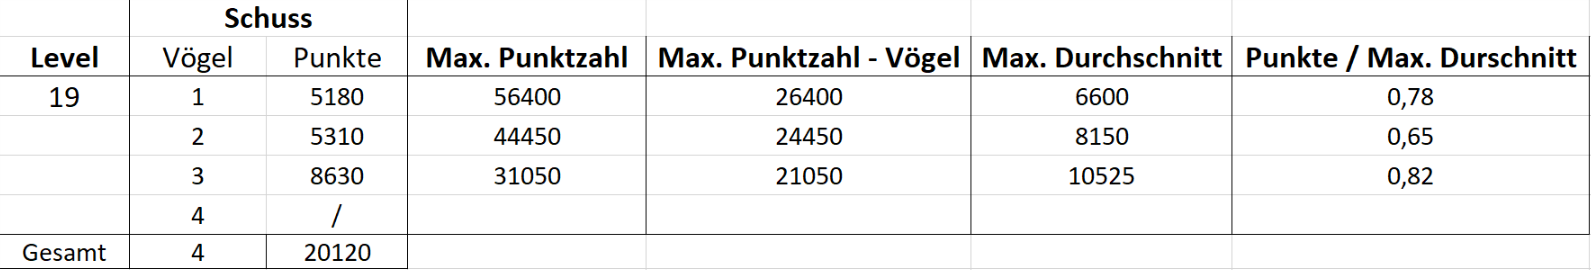
\includegraphics[width=1\textwidth]{Level19}
   \caption{Level 19}
   \label{lvl19}
\end{figure}

\begin{itemize}
\item \textit{Max. Punktzahl}: Maximal zu erreichende Punktzahl des gesamten Levels bevor der Schuss ausgeführt wurde
\item \textit{Max. Durchschnitt}: maximal zu erreichender Durchschnittswert pro Schuss bezogen auf dem momentanen Zustand des Levels 
\end{itemize}

Da unserer Meinung nach alle Schüsse in diesem Level gut waren und wir den 2. Schuss noch an der Grenze zu gut sahen, stellten wir die Regel auf: der Schuss muss mind. 65\% von dem maximal zu erreichenden Durchschnittswert abdecken, um als guten Schuss zu gelten. \\
\\
Ebenso sind wir auch mit dem zweiten Aspekt -- Anzahl der verwendeten Vögel -- vorgegangen und haben einige Szenarien durchgespielt, z.B. war es hervorragend, wenn der Agent höchstens 3 von 4, 3-4 von 5, 4 von 6, 5 von 7, 6 von 8 etc. Vögel verwendet hat. Mit diesen Vergleichen kamen wir dann auf einen Mittelwert von 75\%, d.h. wenn der Agent maximal 75\% der Verfügung gestellten Vögel verbraucht, gilt er als gut. Somit gilt: Je kleiner der Prozentsatz an verwendeten Vögeln ist, desto besser ist die Gesamtbewertung. Daher muss mit dem Wert $Wert2 = 1 - ratio$ gerechnet werden, um eine proportionale Gewichtung zu ermöglichen. \\
\\
Um diese beiden Werte dann in einem gemeinsamen Grenzwert zusammenfassen zu können, muss das Gesamtbild in Betracht gezogen werden. Abbildung \ref{evaluation} veranschaulicht alle Werte in einer Tabelle mit der Formel $0.7 * Wert1 + 0.3 * Wert2$, wobei $Wert1$ das Verhältnis der Punktzahl des einzelnen Schusses -- 1. Aspekt -- und $Wert2$ das Verhältnis für die Anzahl der Vögel -- 2. Aspekt -- darstellt :

\begin{figure}[H]
  \centering
    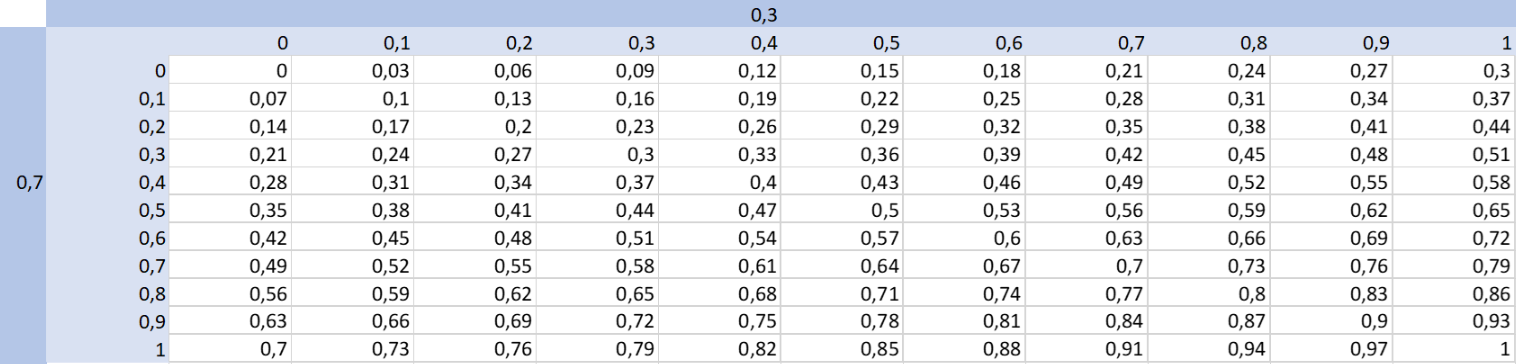
\includegraphics[width=1\textwidth]{EvaluationsWerte}
   \caption{Evaluationswerte}
   \label{evaluation}
\end{figure}

Unsere erste Bedingung ist, dass, falls $Wert1 > 0.65$ gilt, die Gesamtbewertung gut ist, auch wenn alle Vögel verwendet wurden. Daraus folgt: $0.7 * 0.65 + 0.3 * 0 = 0.455$. \\
Diese Grenze lässt sich auch gut auf andere Fälle anwenden, was auch anhand der Tabelle \ref{evaluation} zu sehen ist. Beispielsweise wenn der Agent 80\% aller Vögel verwendet hat, muss der betrachtete Schuss in der vorigen Runde mind. 60\% von der maximal zu erreichenden Durchschnittspunktzahl abgedeckt haben, um noch als \texttt{GOOD} markiert zu werden -- $0.7 * 0.6 + 0.3 * 0.2 = 0.48$. Andernfalls gilt er als \texttt{BAD}. \\ Ein weiteres Beispiel zeigt, wenn der Agent bei dem aktuellen Level zuvor nur 2 von 5 Vögeln benötigt hat, d.h. $Wert2 = 1 - 2/5 = 0.6$, muss die erreichte Punktzahl des Schusses nur 40\% von dem maximalen Durchschnittswert betragen, um die Grenze zum guten Schuss zu überschreiten. \\
Mit etlichen Szenarien waren wir mit dem Gesamtbild zufrieden, weshalb wir die Grenze bei 0.45 bestehen lie\ss en, da es ebenfalls die besten Resultate hervorbrachte.